\documentclass[12pt]{article}

\usepackage{amsthm}
\usepackage{amsmath}
\usepackage{amsfonts}
\usepackage{graphicx}
\usepackage{multirow}
\usepackage{url}
\usepackage{bbm}
\usepackage{float}

\graphicspath{ {images/}{figs/}{figs/node_svm/} }
\usepackage{listings}
\lstset{
  basicstyle=\ttfamily,
  columns=fullflexible,
  frame=single,
  breaklines=true,
}

\theoremstyle{definition}
\newtheorem{definition}{Definition}

\title{{\small{Machine Learning and Algorithms for Data Mining} \\
Assessment 2\footnote{Word count: 2499 --- Computed using TexCount}} \\
\textit{Analysis of graph-structured data}}
\author{Sebastian Borgeaud dit Avocat}

\begin{document}
\maketitle

\begin{abstract}
	In this report, I explore different algorithms that solve the task of transductive classification on a graph and report their accuracy on the Cora dataset \cite{cora}. First, I present a simple baseline method based on support vector machines that only uses the features available at individual nodes. Next, I propose two methods that incorporate the features of neighbouring nodes by averaging over them. As expected, incorporating knowledge about the graph structure gives a significant improvement in classification accuracy, even when incorporated in a simple way. Finally, I reimplement two state-of-the-art methods: Graph Convolutional Networks \cite{kipf2017semi}, and Graph Attention Networks \cite{velickovic2018graph} which achieve the highest accuracy amongst the tested methods.
\end{abstract}

\section{Main contributions, Key Concepts and Ideas}
\subsection{Introduction}
Many real world datasets occur naturally in the form of graphs: examples from different fields include protein-protein interaction networks in biology \cite{schwikowski2000network}, social networks in sociology \cite{otte2002social}, and scientific collaboration networks \cite{newman2001structure}. I focus on the problem of node classification for citation networks in a transductive setting and present multiple approaches to solve this problem. In the transductive case the entire structure of the network is known at training time but only some of the nodes are labelled. At test time, the task is to to infer the labels of the remaining nodes. This differs from supervised learning in two ways: i) The data points are connected to each other through edges. Using these relations might be helpful for classification. ii) As the entire graph is known at test time, the features of the nodes that will be classified at test time are known in advance. 

\subsection{Related work}
It is generally possible to distinguish between two categories of approaches for graph-based semi-supervised learning: methods based on an explicit Laplacian regularisation cost, and methods based on graph-embeddings.

\bigskip

In the first approach, the problem is seen as a graph-based semi-supervised learning problem, where the label information is smoothed over the graph via some form of explicit graph-based regularisation. Examples of such approaches include the label propagation algorithm (Zhu et.\ al \cite{zhu2002learning}) and manifold regularisation (Belkin et al.\ \cite{belkin2006manifold}).

\bigskip

In the second approach, the problem consists of learning embeddings for the nodes using the local graph structure. The embeddings are then used in a semi-supervised setting to learn the corresponding class labels. For example, DeepWalk (Perozzi et al.\ \cite{perozzi2014deepwalk}) learns embeddings using sampled random walks on the graph. This method is extended with more sophisticated random walk search schemes in LINE (Tang et al.\ \cite{tang2015line}) and node2vec (Grover \& Leskovec \cite{grover2016node2vec}).


\subsection{Cora Dataset}
To evaluate the different models I focus on the Cora dataset\footnote{\url{https://linqs.soe.ucsc.edu/data}} \cite{cora}. The dataset consists of $\textrm{N} = 2708$ nodes representing machine learning publications. Each publication is classified into one of $\textrm{C} = 7$ classes: `Case Based', `Genetic Algorithms', `Neural Networks', `Probabilistic Methods', `Reinforcement Learning', `Rule Learning' or `Theory'. The features associated to each node are a binary bag-of-words feature vector for a vocabulary of $\textrm{F} = 1433$ unique words. Let $\mathbf{X}$ be the $\textrm{N} \times \textrm{F}$ matrix containing the features of the nodes in its rows and let $\mathbf{A}$ be the $\textrm{N} \times \textrm{N}$ adjacency matrix of the graph. The $i^\textsuperscript{th}$ row of $\mathbf{X}$,  $\mathbf{X}_i$, contains the bag-of-words binary vector for node $i$. The edges are directed and represent citations, where an edge $\mathit{pub_1} \to \mathit{pub_2}$ means that publication $\mathit{pub_2}$ is cited in publication $\mathit{pub_1}$. The papers were selected in such a way that every paper cites or is cited by at least one other paper. 

\bigskip

In particular, I use the data split introduced by Kipf and Welling \cite{kipf2017semi}: 140 training nodes (about 6.7\% of the nodes), 500 validation nodes and 1000 test nodes. Let $\mathbf{X}_{L}$ and $\textbf{y}_L$ be the matrices containing the features and the labels of the labelled nodes. Furthermore, the edge orientations are ignored.

\subsubsection{Node degree distribution}
The distribution of node degrees is plotted in figures \ref{fig/node_degrees} and \ref{fig/node_degrees_truncated}. Most nodes have few edges, with 59.9\% of the nodes having 3 edges or less and over 96.5\% having 10 or less. There seems to be one outlier publication with 168 edges, whereas the second most citing paper has only 78 edges.

\begin{figure}[H]
	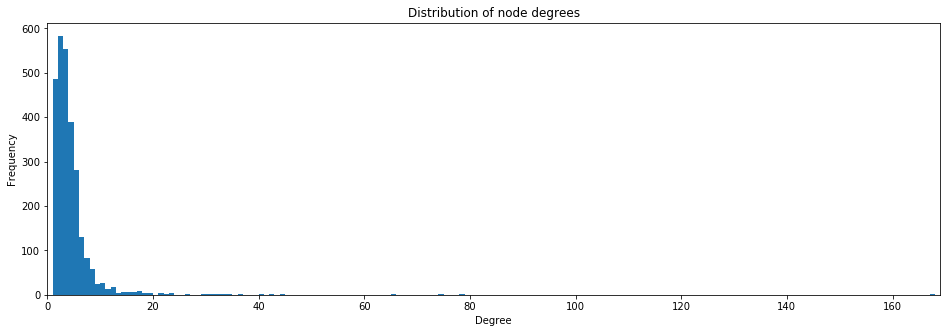
\includegraphics[width=0.8\textwidth]{node_degrees}
	\centering
	\caption{Distribution of the node degrees in the Cora dataset}
	\label{fig/node_degrees}
\end{figure}

\begin{figure}[H]
	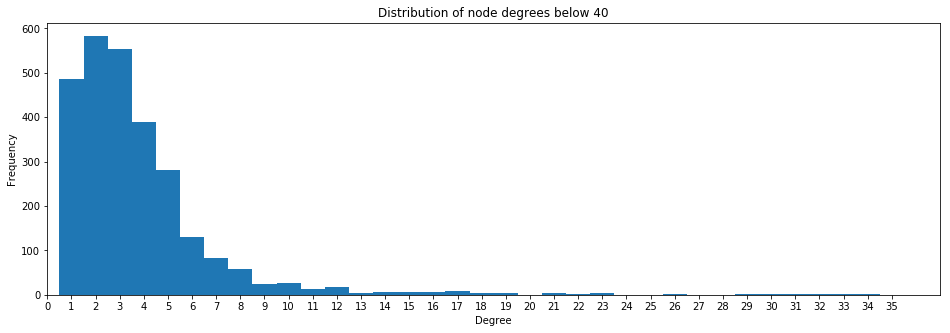
\includegraphics[width=0.8\textwidth]{node_degrees_truncated}
	\centering
	\caption{Distribution of the node degrees with degree below 40. This includes 2701 of the 2708 publications, or above 99.7\% of the nodes.}
	\label{fig/node_degrees_truncated}
\end{figure}

\subsubsection{Clusters}
Furthermore, it is interesting to explore how densely clustered the network is. Using a simple breath-first search algorithm, I found that there are a total of 78 clusters. However, most of the nodes are in the largest cluster which contains 2485 nodes, that is about 91.7\% of the nodes. The full distribution of cluster sizes is shown in table \ref{table/cluster_sizes}.
\begin{table}[h]
\centering	
{\renewcommand{\arraystretch}{1.4} %<- modify value to suit your needs
\begin{tabular}{ c | c c c c c c c c c}
\textbf{Cluster size} & 2  & 3 & 4 & 5 & 6 & 8 & 9 & 26 & 2485 \\
\hline
\textbf{Frequency} 	  & 57 & 7 & 6 & 3 & 1 & 1 & 1 & 1  & 1 \\
\end{tabular}
}
\caption{Distribution of cluster sizes in the Cora dataset.}
\label{table/cluster_sizes}
\end{table}


\section{Methods}
In this section, I present the algorithms I implement to solve the classification task.

\subsection{SVM on node features (node SVM)}
The first method provides a simple baseline model and doesn't incorporate any information about the structure of the network. The problem reduces to a supervised learning task, which I solve with a support vector machine (SVM) trained on the features of the nodes.
\bigskip

Using scikit-learn\footnote{\url{http://scikit-learn.org/}} \cite{scikit-learn} I train a SVM on the labelled training nodes. The trained model is then used to predict the class labels of the test publications.

\subsection{SVM with neighbour features (average SVM)}
\label{section/average_svm}
For the second approach, I incorporate information about the graph structure into the SVM model. To do this, I combine the neighbours of a node by taking the average of their features and concatenating the resulting vector to the feature vector of the node itself. That is, we train the SVM on the features $\mathbf{X}'$ where for each node $i$,
\[
	\mathbf{X}_i' = \big[\mathbf{X}_i \big\vert \big\vert \mathbf{X}^{\mathit{neighbours}}_i \big]
\]
where
\[
	\mathbf{X}^{\mathit{neighbours}}_i  = \frac{1}{\left\vert \mathcal{N}(i) \right\vert} \sum_{j \in \mathcal{N}(i)} \mathbf{X}_j,
\]
$\mathcal{N}(i)$ is the set containing the neighbour nodes of node $i$, and $[\cdot \vert\vert \cdot ]$ denotes vector concatenation. Note that $\mathbf{X}'$ is a $\textrm{N} \times 2 \textrm{F}$ matrix and thus contains twice as many entries as $\mathbf{X}$.

\subsection{Multilayer perceptron (average MLP)}
Next, I train a simple multilayer perceptron using the concatenated features $\mathbf{X}'$. The network consists of two fully-connected layers. The first layer consists of 64 hidden units and has a ReLU activation function. The second layer consists of $C=7$ output units, to which the softmax activation is applied. The output gives a probability distribution over the 7 classes. Furthermore, as there are only few training nodes, I make heavy use of two regularisation techniques: i) Dropout \cite{srivastava2014dropout} applied to the input layer and to the hidden layer, and ii) L2 regularisation on the weights of the first hidden layer.

\subsection{Graph Convolutional Network (GCN)}
The fourth algorithm I implement is the Graph Convolutional Network, presented by Kipf and Welling \cite{kipf2017semi}. Here, the graph structure is encoded directly using a neural network $f(\mathbf{X}, \mathbf{A})$ where $\mathbf{X}$ is the usual feature matrix and $\mathbf{A}$ is the adjacency matrix. The model is trained on a single supervised loss $\mathcal{L}_0$. However, as the adjacency matrix is also inputted to the network, the gradient information is distributed back from $\mathcal{L}_0$ to all nodes and therefore representations are learned for nodes with and without labels \cite{kipf2017semi}.

\bigskip

A Graph Convolutional Network (GCN) is a neural network with the following layer-wise propagation rule: the activations in each layer $\mathbf{H}^{(l)}$ are computed as
\[
\mathbf{H}^{(l+1)} = \sigma \big( \tilde{\mathbf{D}}^{-\frac{1}{2}} \tilde{\mathbf{A}} \tilde{\mathbf{D}}^{-\frac{1}{2}} \mathbf{H}^{(l)} \mathbf{W}^{(l)}\big)
\]
Here, $\tilde{\mathbf{A}} = \mathbf{A} + \mathbf{I}_\textrm{N}$ is the adjacency matrix with added self-connections and $\tilde{\mathbf{D}}$ is a diagonal  matrix with $\tilde{D}_{ii} = \sum_{j} \tilde{A}_{ij}$. $\mathbf{W}^{(l)}$ are the trainable neural network weights in layer $l$. Finally, $\sigma(\cdot)$ is an activation function.

\bigskip

For the Cora dataset, the authors present a 2 layer GCN with a ReLU activation in the first layer and a softmax activation in the second layer. The computation of the forward pass of the neural network can therefore be described concisely as
\[
f(\mathbf{X},\mathbf{A}) = \textrm{softmax}\big(\hat{\mathbf{A}}\ \textrm{ReLU}\big( \hat{\mathbf{A}} \mathbf{X} \mathbf{W}^{(0)} \big)\ \mathbf{W}^{(1)} \big)
\]
where \begin{itemize}
	\item $\hat{\mathbf{A}} = \tilde{\mathbf{D}}^{-\frac{1}{2}} \tilde{\mathbf{A}} \tilde{\mathbf{D}}^{-\frac{1}{2}}$,
	\item $\mathbf{W}^{(0)}$ is an $\textrm{N} \times \textrm{H}$ weight matrix, where $\textrm{H}$ is the number of nodes in the hidden layer,
	\item $\mathbf{W}^{(1)}$ is an $\textrm{H} \times \textrm{C}$ weight matrix, where $\textrm{C} = 7$ is the number of classes,
	\item the ReLU activation function just clips the input to 0,
\[
\textrm{ReLU}(x) = \max(0, x)
\]
	\item and the softmax activation computes for each component $x_i$
\[
\textrm{softmax}(x_i) = \frac{\exp(x_i)}{\sum_j \exp(x_j)}
\]


\end{itemize} During training the cross-entropy loss 
\[
\mathcal{L} = - \sum_{l \in \mathbf{y}_L} \sum_{c=1}^{C} \mathbbm{1}(
\textbf{y}_{L}^{(l)} = c) \ln f(\mathbf{X},\mathbf{A})_{lc}
\]
is minimised over all labelled examples $\textbf{y}_L$ using gradient descent. Dropout \cite{srivastava2014dropout} is applied to the input features and to the output of the first layer to reduce overfitting.

\subsection{Graph Attention Networks}
The final method I explore is the Graph Attention Network (GAT) proposed by Veli{\v{c}}kovi{\'{c}} et al.\ \cite{velickovic2018graph}. The GAT is based on an attention mechanism which gives the neural network the ability to learn on which part of the input to focus. More specifically, the GAT uses self-attention: the attention mechanism is used to compute a representation of a single sequence. The main idea behind the algorithm is to compute a hidden representation (also called an embedding) for each node in the graph by attending over all its neighbours using self-attention. That is, the network computes an embedding for each node using the nodes in its neighbourhood and by choosing how much attention to pay to each individual neighbour using the self-attention mechanism.

\bigskip

The GAT architecture is best described in terms of its layers. In each layer, the input features $\textbf{X}$ are first linearly transformed into $\textbf{X}' = \textbf{X}\textbf{W}$ where $\mathbf{W}$ is a $\textrm{F} \times \textrm{F}'$ weight matrix. Thus, each node feature vector $\mathbf{h}_i = \mathbf{X}_i$ is linearly transformed to a feature vector $\mathbf{h}'_i = \mathbf{X}'_i = \mathbf{h}_i \textbf{W}$ of length $F'$. Then, self-attention is performed on the nodes by applying a shared attentional mechanism defined as a function $a: \mathbb{R}^{F'} \times \mathbb{R}^{F'} \to \mathbb{R}$. This function maps two transformed input feature vectors to a real attention coefficient:
\[
e_{ij} = a(\mathbf{h}'_i, \mathbf{h}'_j) = a(\mathbf{h}_i \textbf{W}, \mathbf{h}_j \textbf{W})
\]

Intuitively, $e_{ij}$ indicates how important the features of node $j$ are to node $i$. To inject graph structural information, we attend over the direct neighbours of $i$, including $i$ itself. Hence, we have that
\begin{equation*}
e_{ij} = \begin{cases}
				a(\mathbf{h}_i \textbf{W}, \mathbf{h}_j \textbf{W}) &\text{if $A_{ij} = 1$ or $i = j$}\\
				0 &\text{otherwise}
			\end{cases}
\end{equation*}
Then, the coefficients are normalised using the softmax function:
\[
\alpha_{ij} = \textrm{softmax}(e_{ij}) = \frac{\exp(e_{ij})}{\sum_{k \in \mathcal{N}(i)} \exp(e_{ik})}
\]
This is done for every pair of nodes $i$ and $j$ to obtain an $\textrm{N} \times \textrm{N}$ matrix $\alpha_{ij}$ of attention coefficients.

\bigskip

The attention mechanism is defined to be a single-layer neural network, parametrised by weights $\textbf{a}$, and using a LeakyReLU nonlinearity: 
\[
\textrm{LeakyReLU}_{\alpha}(x) = 
	\begin{cases}
		x &\text{if $x \ge 0$}\\
		\alpha x &\text{otherwise}
	\end{cases}
\]
The attention coefficients can therefore be described concisely as
\[
\alpha_{ij} = \frac{\exp \big( \textrm{LeakyReLU}\big( \textbf{a}^T \big[ \mathbf{h}_i \textbf{W} \vert\vert \mathbf{h}_j \textbf{W} \big] \big) \big)}
{
\sum_{k \in \mathcal{N}(i)} \exp \big( \textrm{LeakyReLU}\big( \textbf{a}^T \big[ \mathbf{h}_i \textbf{W} \vert\vert \mathbf{h}_k \textbf{W} \big] \big) \big)
}
\]
Next, we use the attention coefficients to compute a linear combination of the transformed features and apply a nonlinearity. This gives the final output of the layer
\[
g_i = \sigma \big( \sum_{j \in \mathcal{N}(i)} \alpha_{ij} \mathbf{h}_j \textbf{W} \big)
\]
Furthermore, we can apply multi-head attention to stabilise the learning process. Instead of using a single attention mechanism, we use $K_a$ independent attention heads, concatenating their output:
\[
g_i = {\Big\vert\Big\vert}_{k=1}^{K_a} \sigma \big( \sum_{j \in \mathcal{N}(i)} \alpha_{ij}^k \mathbf{h}_j \textbf{W}^k \big)
\]
Note that in this case the output feature vectors will have size $K_a F'$.

\bigskip

Veli{\v{c}}kovi{\'{c}} et al.\ propose a GAT network consisting of two graph attention layers. The first layer has $K_a=8$ parallel attention heads and computes a hidden representation of features of size $F'=8$. The nonlinearity used is the exponential linear unit ELU:
\[
\textrm{ELU}_{\alpha}(x) = 
	\begin{cases}
		x &\text{if $x \ge 0$}\\
		\alpha (\exp(x) - 1) &\text{otherwise}
	\end{cases}
\]
The second layer has $C$ features, a single activation head $K_a=1$, and uses a softmax activation.

\bigskip

L2 regularisation is added and Dropout \cite{srivastava2014dropout} is applied to the layers' inputs and to the attention coefficients. Thus at each training epoch, a node is only exposed to a sample of its neighbourhood. 

\section{Results \& analysis}
The results obtained with the various methods described above are shown in table \ref{table/all_results}.
\begin{table}[H]
\centering	
{\renewcommand{\arraystretch}{1.4} %<- modify value to suit your needs
\begin{tabular}{ c c c }
\textbf{Method} & \multicolumn{2}{c}{\textbf{Accuracy}} \\
  & validation & test \\
%\cline{2-3}
\noalign{\vskip 5mm}    
linear node SVM & 0.558 & 0.583 \\
RBF node SVM & 0.566 & 0.576 \\
\hline
linear average SVM & 0.714 & 0.728 \\
RBF average SVM & 0.716 & 0.733 \\
\hline
average MLP & 0.762 & 0.769 \\
\hline
GCN & \textbf{0.785} & \textbf{0.802} \\
\hline
GAT & 0.769 & 0.794 \\
\end{tabular}
}
\caption{Test and validation accuracy obtained using the different models.}
\label{table/all_results}
\end{table}

\bigskip 
Next, I go through the implementation details for each of the methods presented  and explain how the hyper-parameters are optimised.

\subsection{SVM on node features}
Using the 500 validation nodes I optimise the hyper-parameters of the SVM by using a grid-search approach over a range of parameters. I consider both linear and a radial basis function (RBF) kernels. For the linear kernel $C$ is taken at regular intervals on a logarithmic scale ranging from $2^{-15}$ to $2^3$. For the RBF kernel, $C$ is taken from a logarithmic scale ranging from $2^{-15}$ to $2^5$ and $\gamma$ is taken from the range $2^{-15}$ to $2^3$. The validation accuracy obtained for these hyper-parameters ranges are presented in figures \ref{fig/node_svm_linear_reg} and \ref{fig/node_svm_rbf_reg}. The validation accuracy is maximised at 56.6\%, obtained with the RBF kernel, $C=1.86$ and $\gamma=2^{-7}$. 

\bigskip

Although significantly below the current state-of-the-art accuracy, this provides a simple baseline accuracy on the test nodes of 57.6\%. This is significantly better than a random baseline, which would have an expected accuracy of $\frac{1}{7}$ (14.3\%). This suggests that, rather unsurprisingly, a lot of the information required for classification is contained in the bag-of-words vectors. 

\begin{figure}[H]
	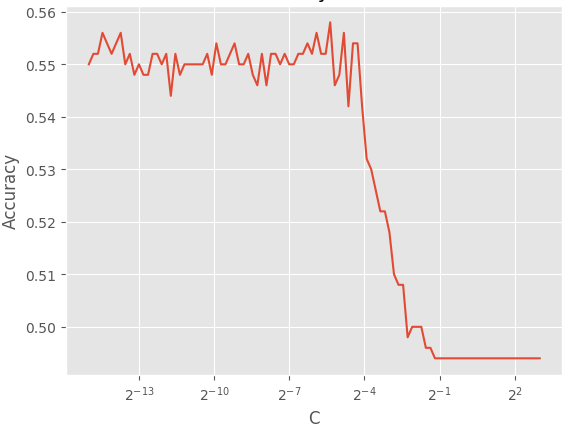
\includegraphics[width=0.4\textwidth]{node_svm/linear_reg}
	\centering
	\caption{Validation accuracy obtained for various values of $C$ for the SVM with a linear kernel trained on the node features alone. The best validation accuracy is obtain at $C=0.024$, with a validation accuracy of 55.8\%.}
	\label{fig/node_svm_linear_reg}
\end{figure}
\begin{figure}[H]
	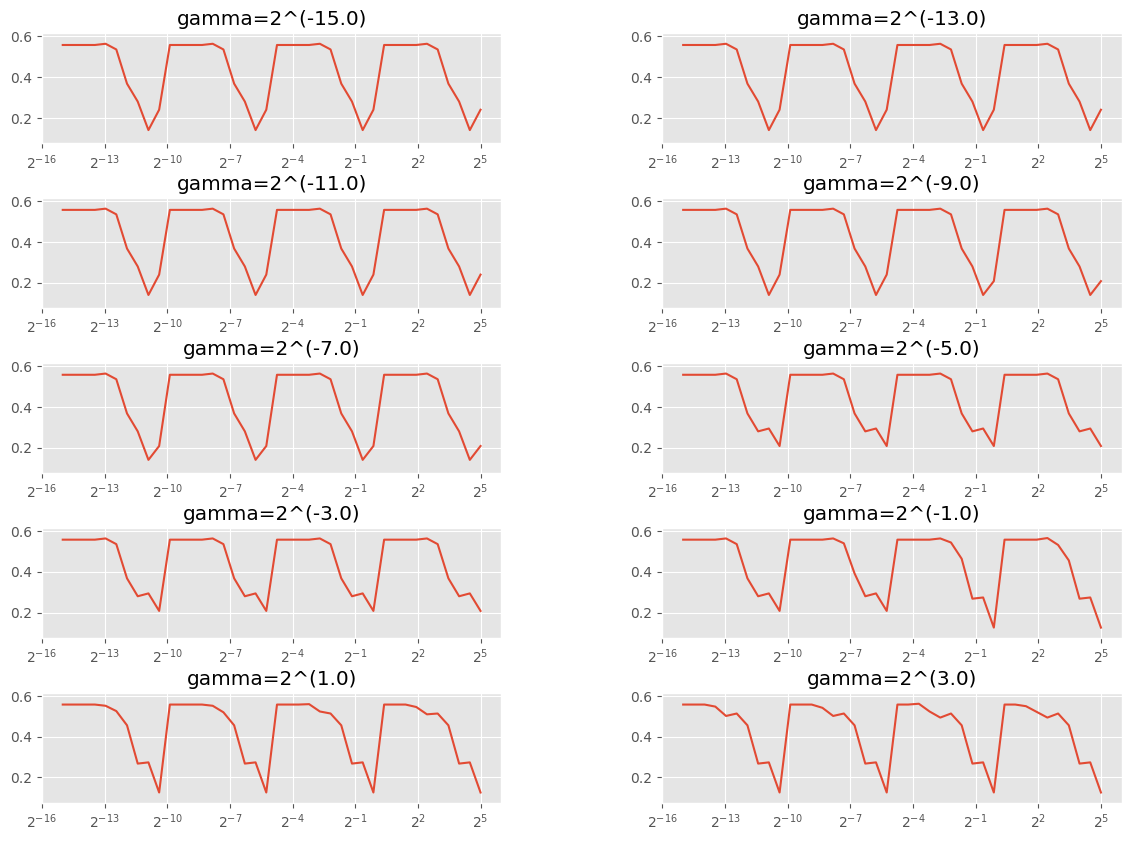
\includegraphics[width=0.7\textwidth]{node_svm/rbf_reg}
	\centering
	\caption{Validation accuracy obtained for various values of $C$ and $\gamma$ for the SVM with an RBF kernel trained on the node features alone. The best validation accuracy is obtain at $C=1.86$ and $\gamma=2^{-7}$, with a validation accuracy of 55.6\%.}
	\label{fig/node_svm_rbf_reg}
\end{figure}

\subsection{Average features SVM}
I train the second SVM this time using the concatenated features $\mathbf{X}'$. I consider both linear and a RBF kernels. The validation accuracies are presented in figures \ref{fig/average_svm_linear_reg} and \ref{fig/average_svm_rbf_reg}. Again, the RBF kernel performs slightly better with a validation accuracy of 71.6\% compared to 71.4\% for the linear kernel. Using the best hyper-parameters with the RBF kernel: $C=5.411$ and $\gamma = 2^{-9}$, I obtain an accuracy of 73.3\% on the test nodes.

\begin{figure}[H]
	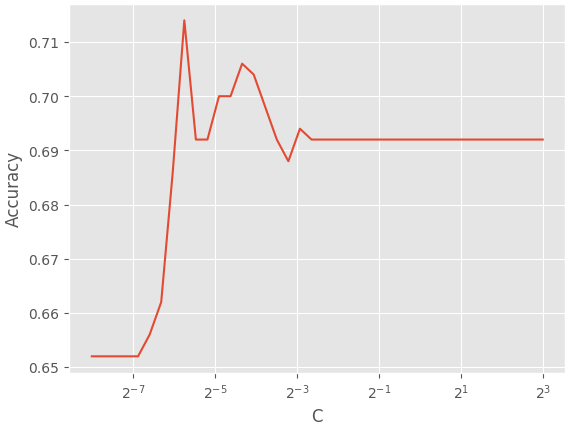
\includegraphics[width=0.4\textwidth]{average_svm/linear_reg}
	\centering
	\caption{Validation accuracy obtained for various values of $C$ for the SVM with a linear kernel trained on the node features and the average neighbouring features. The best validation accuracy is obtain at $C=0.018$, with a validation accuracy of 7.14\%.}
	\label{fig/average_svm_linear_reg}
\end{figure}
\begin{figure}[H]
	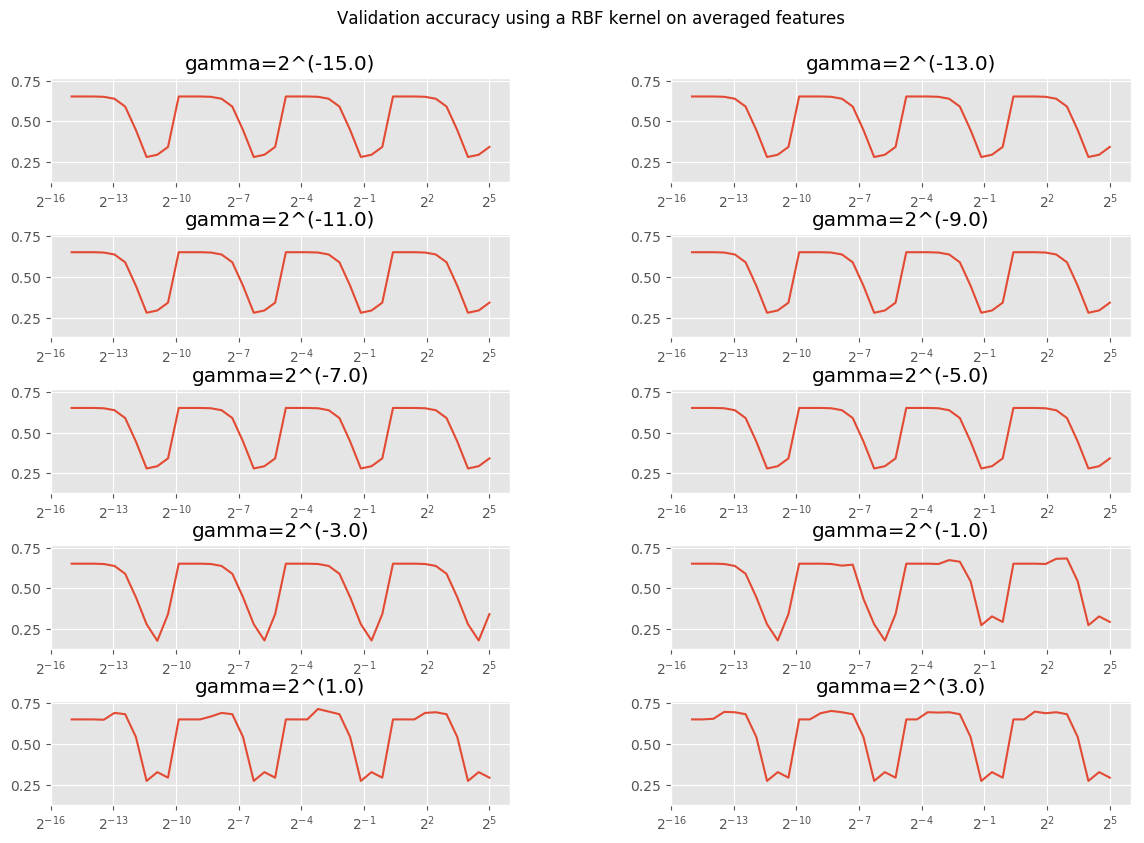
\includegraphics[width=0.7\textwidth]{average_svm/rbf_reg}
	\centering
	\caption{Validation accuracy obtained for various values of $C$ and $\gamma$ for the SVM with an RBF kernel trained on the node features and the averaged neighbouring features. The best validation accuracy is obtain at $C=5.411$ and $\gamma=2^{-9}$, with a validation accuracy of 71.6\%.}
	\label{fig/average_svm_rbf_reg}
\end{figure}

\bigskip

This is a significant improvement over the accuracy obtain with the SVM trained on the features of each node individually. This shows that incorporating knowledge about the graph structure does indeed improve the classification accuracy significantly even when incorporated only in a very simplistic way, i.e.\ by only considering the direct neighbours and averaging their features.

\subsection{Multilayer perceptron}
To find the optimal hyper-parameters, I again use a grid search method, validating the accuracy using the 500 validation nodes. The network is trained using every possible combination of parameters with \texttt{batch\_size} in [32, 64, 128, 140], \texttt{num\_epochs} in  [50, 100, 200, 400], \texttt{dropout\_p} in  [0.0, 0.1, 0.2, 0.4, 0.6] and $\lambda$ in  [0.05, 0.005, 0.001, 0.0001] where $\lambda$ is the L2 regularisation weight. The best validation accuracy of 76.2\% was obtained using the entire training set in a single batch, trained over 400 epochs with a dropout rate of 0.6 and setting $\lambda = 0.0001$. Using these hyper-parameters I obtain a test accuracy of 76.9\%. Figure \ref{fig/mlp_training} shows the loss and accuracy at training time.
\begin{figure}[H]
	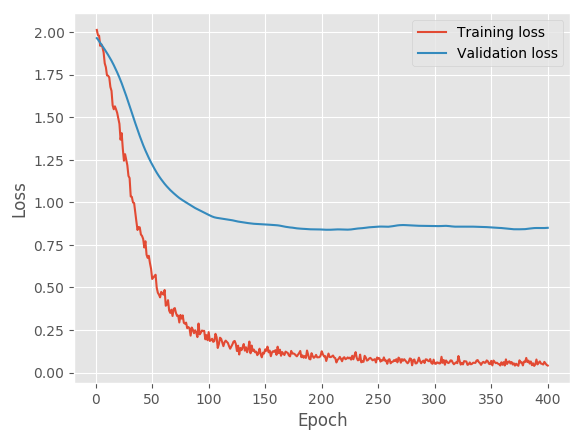
\includegraphics[width=0.49\textwidth]{mlp/loss}
	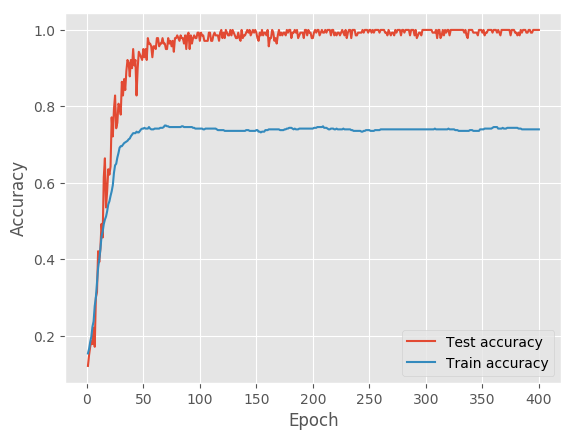
\includegraphics[width=0.49\textwidth]{mlp/acc}
	\centering
	\caption{Accuracy and loss obtained during training of the MLP using the optimised hyper-parameters.}
	\label{fig/mlp_training}
\end{figure}

\bigskip

The multilayer perceptron therefore performs better than the SVM trained on the same input features. This could be explained by the higher complexity of the MLP compared to the SVM.

\subsection{Graph Convolutional Network}

I implement the GCN model using TensorFlow with the optimised hyper-parameters presented by the authors. The model is trained over 200 epochs using the Adam optimiser \cite{kingma2014adam}. The optimal learning rate was found to be 0.01. The weights are initialised using a Glorot initialization \cite{glorot2010understanding}. Furthermore, the input feature vectors are row-normalized. The dropout rate was set to $p=0.5$, the L2 regularisation weight to $\lambda=0.0005$. The number of hidden inputs was set to 16. Averaging the result of 10 runs, I obtain a validation accuracy of 78.5\% and a test accuracy of 80.3\%.

\bigskip

The GCN gives a significant improvement over the MLP. This could be accounted for by multiple reasons. First, the graph structure is incorporated in a more principled way, using the adjacency matrix and the degree matrix of the network. Second, as the network consists of two layers, it has the ability to incorporate information not only from the direct neighbours of a node but also from the neighbours of the neighbours of a node.

\subsubsection{Hidden layer visualisation}

The activations in the hidden layer of the GCN can be visualised using a dimensionality reduction technique. Following the approach taken by Kipf and Welling, I use t-SNE \cite{maaten2008visualizing} to reduce the 16-dimensional hidden activation to 2 dimensions. Figure \ref{fig/gcn_tsne} shows the resulting vectors.

\begin{figure}[h]
	\includegraphics[width=1.0\textwidth]{gcn/visualisation_tsne}
	\centering
	\caption{Activations in the hidden layer of the GCN, after reducing their dimensionality using t-SNE for the training, validation and test nodes. As expected, the network is able to learn to discern the training nodes well and this generalises to the validation and test nodes. Different colours represent different classes.}
	\label{fig/gcn_tsne}
\end{figure}

\subsection{Graph Attention Network}
Similarly as for the GCN, I use the hyper-parameters presented by the author but reimplement the network in TensorFlow. The regularisation weight is set to $\lambda = 0.0005$ and the dropout rate is set to $p=0.6$. The Adam optimiser \cite{kingma2014adam} is used with a learning rate of $\textit{lr} = 0.005$. The model is trained over 100 epochs, each with a single batch containing all 2708 nodes.

I obtain a validation accuracy of 76.9\% and a test accuracy of 79.4\%, which is below the accuracy reported by the authors (83.0\%). This discrepancy could be explained by small differences between the two implementations of the algorithm. 

\subsubsection{Embeddings visualisation}
Using t-SNE we can reduce the dimensionality of the learned embeddings, i.e.\ the output of the first layer of the GAT. Reducing to 2 dimensions I plot the embeddings in a plane, as shown in figure \ref{fig/gat_tsne}.
\begin{figure}[h]
	\includegraphics[width=1.0\textwidth]{gat/visualisation_tsne}
	\centering
	\caption{Visualisation of the learned embeddings by the GAT. The dimensionality of the embeddings is reduced from 64 to 2 using t-SNE. The embeddings are shown for the training, validation and test nodes. As expected, the network is able to learn to discern the training nodes well and this generalises to the validation and test nodes. Different colours represent different classes.}
	\label{fig/gat_tsne}
\end{figure}

\section{Conclusion}
	I implemented 5 different approaches to solve the task of transductive classification on the Cora dataset \cite{cora}. Experiments show that a simple baseline method using the node features alone is sufficient to obtain significantly better results than using a random baseline. Using information given by the graph structure by concatenating the average of the neighbouring node features to the features of a node itself did increase the accuracy significantly. My implementation of the more sophisticated approaches, i.e.\ the GCN and the GAT obtained the best results, closely matching the current state-of-the-art results for this dataset.	
\bibliography{bib}
\bibliographystyle{unsrt}


\end{document}